\subsection{Current Sports Booking Applications}
\label{sub:current_sports_booking_applications}

Our application will allow searching across multiple organisations, locations,
times and sports to provide available bookings. There are currently no
applications that allow searching across multiple organisations' facilities for
available sports bookings. There are, however, web applications for specific
organisations which:
\begin{itemize}
        \item have multiple locations, each with many available sports to play,
        \item have a single location with many sports to play,
        \item have multiple locations with a single sport to play.
\end{itemize}
There are also web applications which allow for searching of different
facilities but offer no information on available bookings beyond providing
contact information for each facility.

\subsubsection{University Of Birmingham Sport}
\label{ssub:university_of_birmingham_sport}

The University Of Birmingham has an online booking system for numerous sports available to play at facilities at its campus in Edgbaston\cite{UOBSport}. This site allows search by location, type of activity and time. Once the user has entered their search criteria, a list of ``activities'' are returned. The user then selects an activity and is shown a timetable indicating at what time this activity is available. The activity can then be booked directly on the website.

\begin{figure}[ht]
\centering
\begin{subfigure}[b]{0.4\textwidth}
                   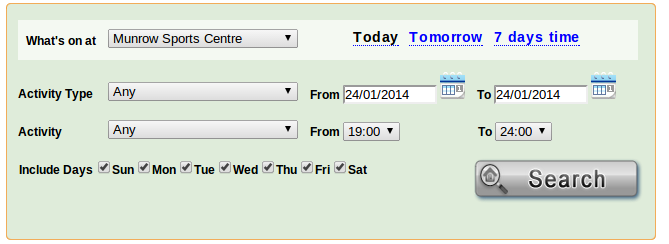
\includegraphics[width=\textwidth]{img/UoBSearch.png}
                   \caption{Search form}\label{fig:UoBSearch}
\end{subfigure}%
\qquad
\begin{subfigure}[b]{0.4\textwidth}
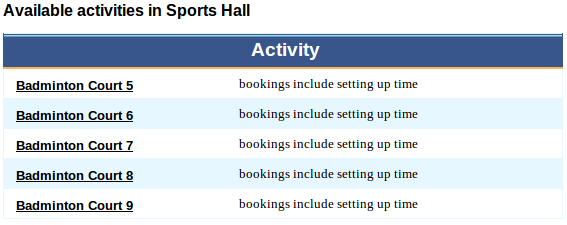
\includegraphics[width=\textwidth]{img/UoBResults.png}
\caption{List of results}\label{fig:UoBResults}
            \end{subfigure}
            \qquad
            \begin{subfigure}[b]{0.7\textwidth}
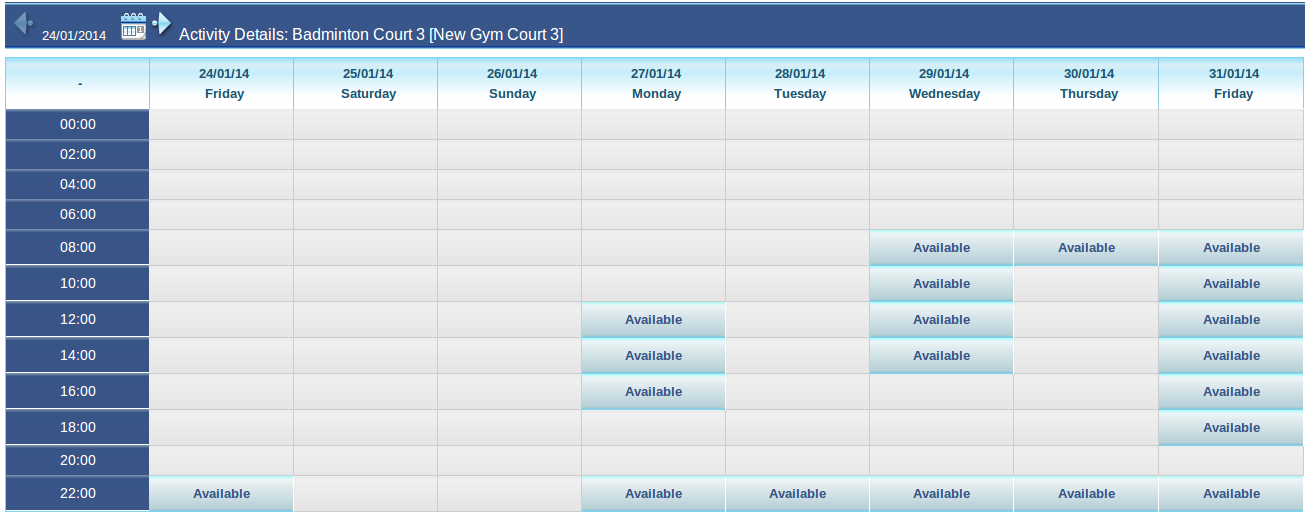
\includegraphics[width=\textwidth]{img/UoBTimetable.png}
\caption{Timetable of available bookings}\label{fig:UoBTimetable}
\end{subfigure}
\caption{The booking interface for University of Birminghan Sport}\label{fig:animals}
\end{figure}

\paragraph{Strengths}

\begin{itemize}
        \item The search form has tick boxes to filter out particular days of the week. A user may only know which days of the week they want to play a sport rather than exact dates. This feature gives the user a quick way to search for this.
        \item There are quick links on the form to change the date ranges to either today, tomorrow or 7 days time. When a group finishes playing a particular sport one week, they may want to quickly see what is available at the same time the following week; these quick links speed up the process of finding these available bookings.
        \item It is possible to search solely by time, leaving all sport and location fields blank. If the user knows they want to play a sport at a particular time, but would like to have options on sport and location, the search form in figure~\ref{fig:UoBSearch} allows them to search this way.
\end{itemize}

\paragraph{Weaknesses}

\begin{itemize}
        \item The option to filter by ``activity type'' in the search form is actually a filter for location and many of the locations host a variety of different sports. Furthermore, the names of these locations, such as ``Sports Hall'', often offer no clear indication of which sports are available at a particular location. If the user wants to know what sports are played at a particular venue, they have select that venue and then see which options then appear under the ``Activity'' drop down box of the search form. This is confusing and unintuitive for the user.
        \item For many sports, such as badminton where there are multiple courts available for badminton across several locations, there is no way to simply search by that sport. The user is required to go to each court individually to see what times are available for that court. The user is unlikely to have a court preference and most likely just wants to know at what times they can play badminton; this system offers no quick and easy way to do this.
        \item The timetable results groups times into two hour slots but often each booking slot is one hour long. It will show `available' for a two hour slot when at least one of those two hours is available. Therefore it is impossible to know if the exact hour a user wants to play is available without selecting the containing two hour slot as shown in figure~\ref{fig:UoBTimetableDD}.

\begin{figure}
\begin{center}
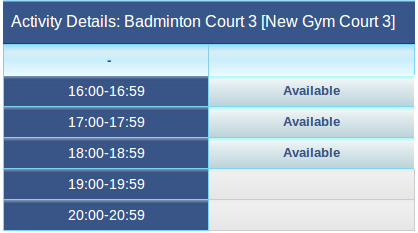
\includegraphics[width=0.4\textwidth]{img/UoBTimetableDD}
\end{center}
\caption{Display when the 18:00 two hour slot is chosen. However, only one of two hours following 18:00 is available}\label{fig:UoBTimetableDD}
\end{figure}

        \item There is no indication of price until you select a booking slot for a particular sport at a particular time.
\end{itemize}

\subsubsection{Aquaterra Leisure Centres}
\label{ssub:aquaterra_leisure_centres}

Aquaterra is a charity funded by Islington Council who manage several leisure centres and other sports facilities in Islington, London. They maintain a website\cite{AquaterraLeisure} where users are able to book at each of these facilities. The booking home page shown in figure~\ref{fig:AquaterraHome} prompts a user to select which of the locations they would like to make a booking at.

\begin{figure}[ht]
\centering
\begin{subfigure}[b]{0.4\textwidth}
                   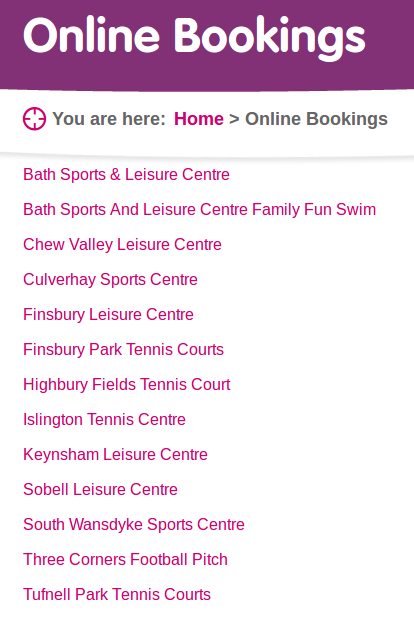
\includegraphics[width=\textwidth]{img/AquaterraHome.png}
                   \caption{Aquaterra booking homepage}\label{fig:AquaterraHome}
\end{subfigure}
\qquad
\begin{subfigure}[b]{0.4\textwidth}
                   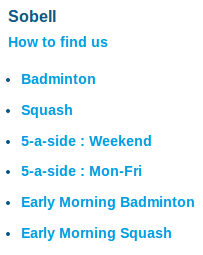
\includegraphics[width=\textwidth]{img/AquaterraSobellHome.png}
                   \caption{Facilities available at Sobell Leisure Centre}\label{fig:AquaterraSobellHome}
\end{subfigure}
\qquad
\caption{The booking interface for Aquaterra Leisure Centres}\label{fig:AquaterraHomeMain}
\end{figure}

The interface for each of the locations varies slightly, but each will generally show a list of available activities at that location that can be selected to display a timetable of available booking slots within the following week for that particular activity. The price is displayed at this point and the booking can then be made directly on the website after choosing a preferred court.

\begin{figure}[ht]
\centering
\begin{subfigure}[b]{0.45\textwidth}
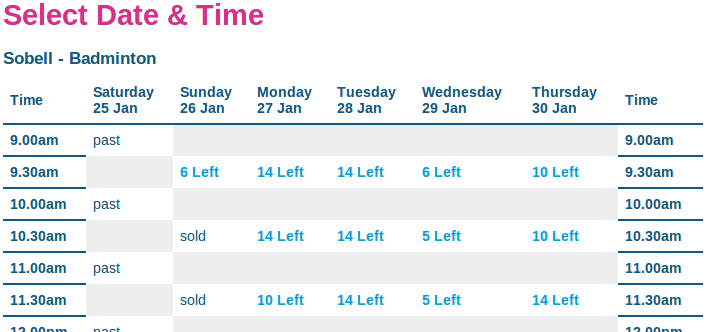
\includegraphics[width=\textwidth]{img/AquaterraSobellBadminton.png}
\caption{Beginning of timetable showing available badminton slots}\label{fig:AquaterraSobellBadminton}
            \end{subfigure}
            \qquad
\begin{subfigure}[b]{0.45\textwidth}
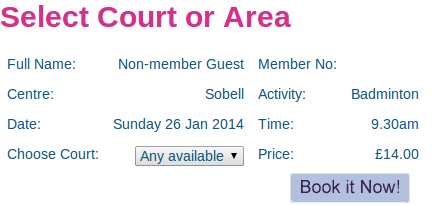
\includegraphics[width=\textwidth]{img/AquaterraSobellConfirm.png}
\caption{Confirmation page for a booking slot showing price and choice of courts available}\label{fig:AquaterraSobellConfirm}
            \end{subfigure}
            \qquad
\caption{The booking interface for badminton at Sobell Leisure Centre}\label{fig:AquaterraSobellBadmintonMain}
\end{figure}

\paragraph{Strengths}

\begin{itemize}
        \item If a user knows the location they wish to play at and the sport they wish to play,  then they can see on one page everything that is available to them in the next week. Rows being coloured alternately and having the time displayed at both sides of the timetable makes it easy for the user to navigate to a particular time slot at a glance.
        \item The timetable for badminton in figure~\ref{fig:AquaterraSobellBadminton} indicates how many courts are available within each slot. If very few courts are available in a preferred time slot, it could indicate to the user that they need to make a quick decision as those courts may soon be booked by someone else. Conversely, if there are many courts available it could indicate to the user that they could delay making a decision on which time to book a court. Providing the user with this information early in the search process could be very helpful.
\end{itemize}

\paragraph{Weaknesses}

\begin{itemize}
        \item When selecting a location from the page in figure~\ref{fig:AquaterraHome}, there is very little indication to the user what sports are available at which location. Therefore if they want to play a particular sport but have no location preference, they are required to go through each option on the homepage to compare what facilities are available for that sport at each location. Furthermore, as each location's page has a slightly different interface, the user has to make sense of each page separately, slowing down their ability to compare information provided for each location.
        \item There is no indication of price until you select a particular sport at a particular time.
\end{itemize}

\subsubsection{London Tennis}
\label{ssub:london_tennis}

London Tennis is a website designed to help tennis players in London find partners to play with, as well as tournaments to play in and courts to play at. The court search feature in figure~\ref{fig:LondonTennisSearch} allows a user to search for a court anywhere in London including options to search by cost of playing, location and type of court. 

\begin{figure}[ht]
\centering
\begin{subfigure}[b]{0.6\textwidth}
                   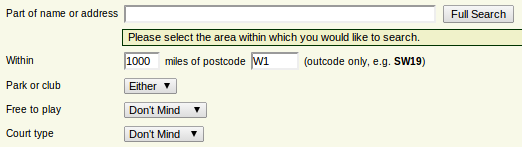
\includegraphics[width=\textwidth]{img/LondonTennisSearch.png}
                   \caption{The search form for looking for a tennis court}\label{fig:LondonTennisSearch}
\end{subfigure}%
\qquad
\begin{subfigure}[b]{0.3\textwidth}
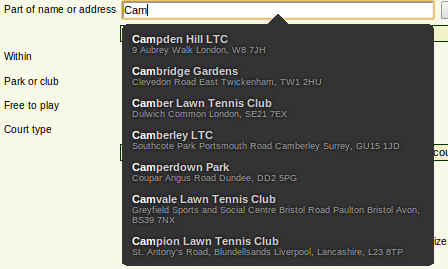
\includegraphics[width=\textwidth]{img/LondonTennisPredict.png}
\caption{Drop down to predict input when typing a name of a court}\label{fig:LondonTennisMap}
            \end{subfigure}
            \qquad
\caption{The search form for London Tennis}\label{fig:LondonTennisSearchMain}
\end{figure}

There is also the option to select courts from a map, as shown in figure~\ref{fig:LondonTennisMap}. Users can filter out courts which are free or not free. However, there are no other interactive features on this map. Once a search is performed, the user is shown a list of courts matching their chosen criteria as seen in figure~\ref{fig:LondonTennisResults}. Once a court is chosen, the user is shown details about the court including exact location, type of court, price and weather predictions for the local area.

\begin{figure}
\begin{center}
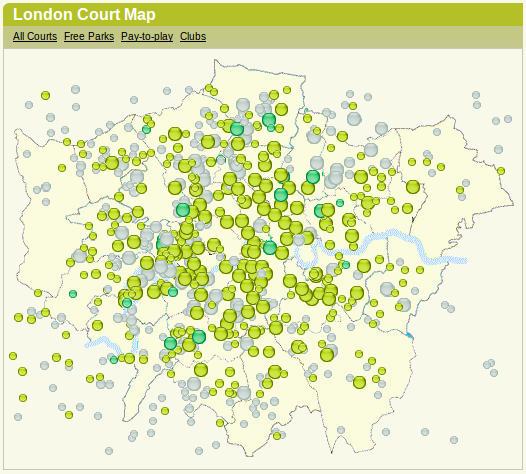
\includegraphics[width=0.7\textwidth]{img/LondonTennisMap.png}
\end{center}
\caption{All courts by location on a map with the ability to filter between free and pay-to-play courts}\label{fig:LondonTennisMap}
\end{figure}

\begin{figure}[ht]
\centering
\begin{subfigure}[b]{0.7\textwidth}
                   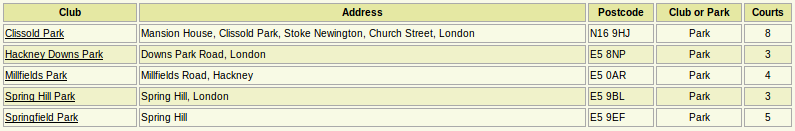
\includegraphics[width=\textwidth]{img/LondonTennisResults.png}
                   \caption{List of courts matching a search}\label{fig:LondonTennisResults}
\end{subfigure}
\begin{subfigure}[b]{0.7\textwidth}
                   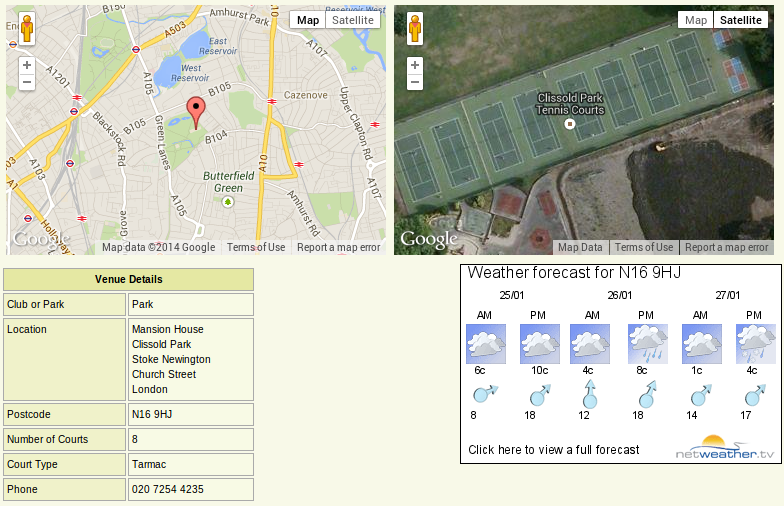
\includegraphics[width=\textwidth]{img/LondonTennisDetails.png}
                   \caption{Details about a chosen court}\label{fig:LondonTennisDetails}
\end{subfigure}
\caption{The displays for results of a search}\label{fig:LondonTennisResultsMain}
\end{figure}

\paragraph{Strengths}
\begin{itemize}
        \item The user is able to show only free courts straight away without having to complete any other aspects of the search. This is in contrast to other sites we have seen so far and allows the user to immediately filter by something that is potentially a deciding factor in choosing a court.
        \item The weather predictions are a useful addition given tennis is very much dependent on good weather.
\end{itemize}

\paragraph{Weaknesses}
\begin{itemize}
        \item The size of the map for searching in figure~\ref{fig:LondonTennisMap} is too small for the number of courts shown on the map, particularly given there is no option to zoom in to more detail on the map. Though the map does give, at a glance, an idea of where courts are concentrated in London, it is difficult to actually select a court due to how close the buttons to select each court are to each other.
        \item There is no information about opening times for any of the courts. Although London Tennis is primarily a service to find court locations rather than provide details about available bookings it would be useful to inform the user of when the courts are even open.
\end{itemize}

\subsubsection{What we can learn}
\label{ssub:what_we_can_learn}

\begin{itemize}
        \item It could be useful to add options to filter by day of the week in addition to buttons that quickly allow searching by times relative to today such as tomorrow or one week from now as this is possibly be one of the main criterias of the users search. 
        \item The naming of options to filter by when searching need to be intuitive and unambiguous otherwise it is difficult  for the user to know how to actually search for what they want.
        \item Using a timetable layout similar to figure~\ref{fig:UoBTimetable} could create difficulties in clearly displaying all available options after a search is done. There may be far more booking slots to display in our app given that our search will be conducted over a greater number of facilities. The screen space available will also be smaller than University of Birmingham has on their website. Therefore we need to think of a clearer way of showing the user the results of a search.
        \item Price is likely to be a factor in a user's decision of what sport to play and where, therefore our application needs to either provide a filter to search by price or clearly indicate the price of a booking option as early as possible when displaying results to a user.
        \item If we are to use a map to display results of a search, it will be difficult given the potentially large number of results to display every option individually on the map, particularly if the map covers a large area. Therefore it may be better to group options together - possibly by colour, or different shapes or picture icons - in order to make it possible to read and navigate through the results.
        \item Weather could be an important factor when a user knows when they would like to play a sport but want to compare what sports are available at that time. When a user is looking at search results for outdoor bookings, it could be useful to display weather predictions for that time, particularly if the search is in the near future as predictions are likely to more accurate for the near future.
\end{itemize}
